\section{逻辑回归之二分类}
\label{sec:chapter4}

\subsection{二分类问题与逻辑回归的引入}

给定数据集：
\[
\left\{\left(x^{(i)},y^{(i)}\right),\;i=1,2,\cdots,m\right\}
\]
其中 $x^{(i)}$ 是一个 $n$ 维向量 $\left(x_0^{(i)},\cdots,x_n^{(i)}\right)^T$，且 $y^{(i)}\in\{0,1\}$，也即是对于输入 $x^{(i)}$，我们将其分类为 $0$ 或 $1$ 两类。试用一模型拟合该分类结果。

鉴于 $y$ 取值的离散性，线性回归在这里不好使了，我们引入逻辑回归的概念。

回忆线性回归的假设函数：$h_\theta(x)=\theta^Tx$，我们在其外套上 $\text{sigmoid}$ 函数，构造逻辑回归的假设函数为：
\[
h_\theta(x)=g\left(\theta^Tx\right)=\frac{1}{1+e^{-\theta^T x}}
\]

\begin{note}
$\text{sigmoid}$ 函数：
\[
g(z)=\frac{1}{1+e^{-z}}
\]
是一个介于 $(0,1)$ 之间的单增 $S$ 形函数。
\end{note}

也就是说，对于一个参数为 $\theta$ 的逻辑回归模型，输入 $x$，得到 $h_\theta(x)=\frac{1}{1+e^{-\theta^Tx}}$ 的预测。我们可以把这个值视为 $x$ 这组数据对应的 $y$ 等于 $1$ 的概率，如果它 $\geqslant 0.5$，则分类为 $1$，否则分类为 $0$. 

又根据 $\text{sigmoid}$ 函数的性质，$h_\theta(x)\geqslant 0.5\iff \theta^Tx\geqslant0$. 所以只要 $\theta^Tx\geqslant0$，就分类为 $1$，否则分类为 $0$；于是乎，$\theta^Tx=0$ 这条线（超平面）被称作决策边界，它将整个空间划分成两块，各自属于一个分类。


\subsection{代价函数}

现在，我们的任务就是从数据集中求解逻辑回归的参数 $\theta$. 仍然采用代价函数的思想——找到使代价最小的参数即可。

广义上来讲，代价函数是这样的一个函数：
\[
J(\theta)=\frac{1}{m}\sum_{i=1}^m\text{Cost}\left(h_\theta(x^{(i)}),y^{(i)}\right)
\]
也就是说用每个数据的估计值 $h_\theta(x^{(i)})$ 和真实值 $y^{(i)}$ 计算一个代价 $\text{Cost}\left(h_\theta(x^{(i)}),y^{(i)}\right)$，比如线性回归中这个代价就是二者差值的平方。

具体到逻辑回归里，这个代价定义为：
\begin{align*}
\text{Cost}\left(h_\theta(x),y\right)&=\begin{cases}-\ln(h_\theta(x))&y=1\\-\ln(1-h_\theta(x))&y=0\end{cases}\\
&=-y\ln(h_\theta(x))-(1-y)\ln(1-h_\theta(x))\\
&=y\ln\left(1+e^{-\theta^Tx}\right)+(1-y)\ln\left(1+e^{\theta^Tx}\right)
\end{align*}

\begin{proof}
上式的来源：

前文已经提到，$h_\theta(x)=\mathbb P(y=1)$，于是 $1-h_\theta(x)=\mathbb P(y=0)$，故：
\[
\mathbb P(y=k)=[h_\theta(x)]^k[1-h_\theta(x)]^{1-k},\quad k\in\{0,1\}
\]
考虑\textbf{极大似然法}，在数据集 $\left\{\left(x^{(i)},y^{(i)}\right),\;i=1,2,\cdots,m\right\}$ 下，似然函数为：
\[
L(\theta)=\prod_{i=1}^m\mathbb P\left(y=y^{(i)}\right)=\prod_{i=1}^m\left[h_\theta(x^{(i)})\right]^{y^{(i)}}\left[1-h_\theta(x^{(i)})\right]^{1-y^{(i)}}
\]
取对数得到：
\[
\ln L(\theta)=\sum_{i=1}^my^{(i)}\ln(h_\theta(x^{(i)}))+(1-y^{(i)})\ln(1-h_\theta(x^{(i)}))
\]
注意到，极大似然法的目标是找到 $L(\theta)$ 或 $\ln L(\theta)$ 的极大值，而逻辑回归的目标是找到 $J(\theta)$ 的极小值，所以自然的，我们直接使用 $\ln L(\theta)$ 来定义 $J(\theta)$：
\[
J(\theta)=-\frac{1}{m}\ln L(\theta)
\]
这个 $\frac{1}{m}$ 对极大值/极小值没有影响，仅是取一下平均罢了。

换句话说，\textbf{逻辑回归的本质是拟合 $y$ 取值的概率，并以极大似然法解之}。
\end{proof}


\subsection{梯度下降解逻辑回归}

我们对逻辑回归定义的代价函数是非常好的：它是一个凸函数。这有助于我们进行梯度下降求解。

为了求偏导，我们先计算：
\begin{align*}
\frac{\partial}{\partial\theta}\text{Cost}(h_\theta(x), y)&=\frac{\partial}{\partial \theta}\left[y\ln\left(1+e^{-\theta^Tx}\right)+(1-y)\ln\left(1+e^{\theta^Tx}\right)\right]\\
&=\frac{-yxe^{-\theta^Tx}}{1+e^{-\theta^Tx}}+\frac{(1-y)xe^{\theta^T x}}{1+e^{\theta^T x}}\\
&=\frac{-yx+(1-y)xe^{\theta^Tx}}{1+e^{\theta^Tx}}\\
&=\left(-y+\frac{1}{1+e^{-\theta^Tx}}\right)x\\
&=(h_\theta(x)-y)x
\end{align*}
于是乎，
\[
\frac{\partial J}{\partial\theta}=\frac{1}{m}\sum_{i=1}^m\left(h_\theta(x^{(i)})-y^{(i)}\right)x^{(i)}
\]
没错，这个偏导的形式和线性回归的偏导形式完全相同！不同的只是 $h_\theta(x)$ 的定义——逻辑回归的假设函数在线性回归的假设函数外套了一层 $\text{sigmoid}$ 函数，也正是这一层 $\text{sigmoid}$ 函数，让我们不能像线性回归那样直接给出解析解，而必须使用梯度下降等方法。

现在我们对其使用梯度下降即可。


\subsection{代码实现}

首先看一下数据的散点图：

\begin{figure}[H]
    \centering
    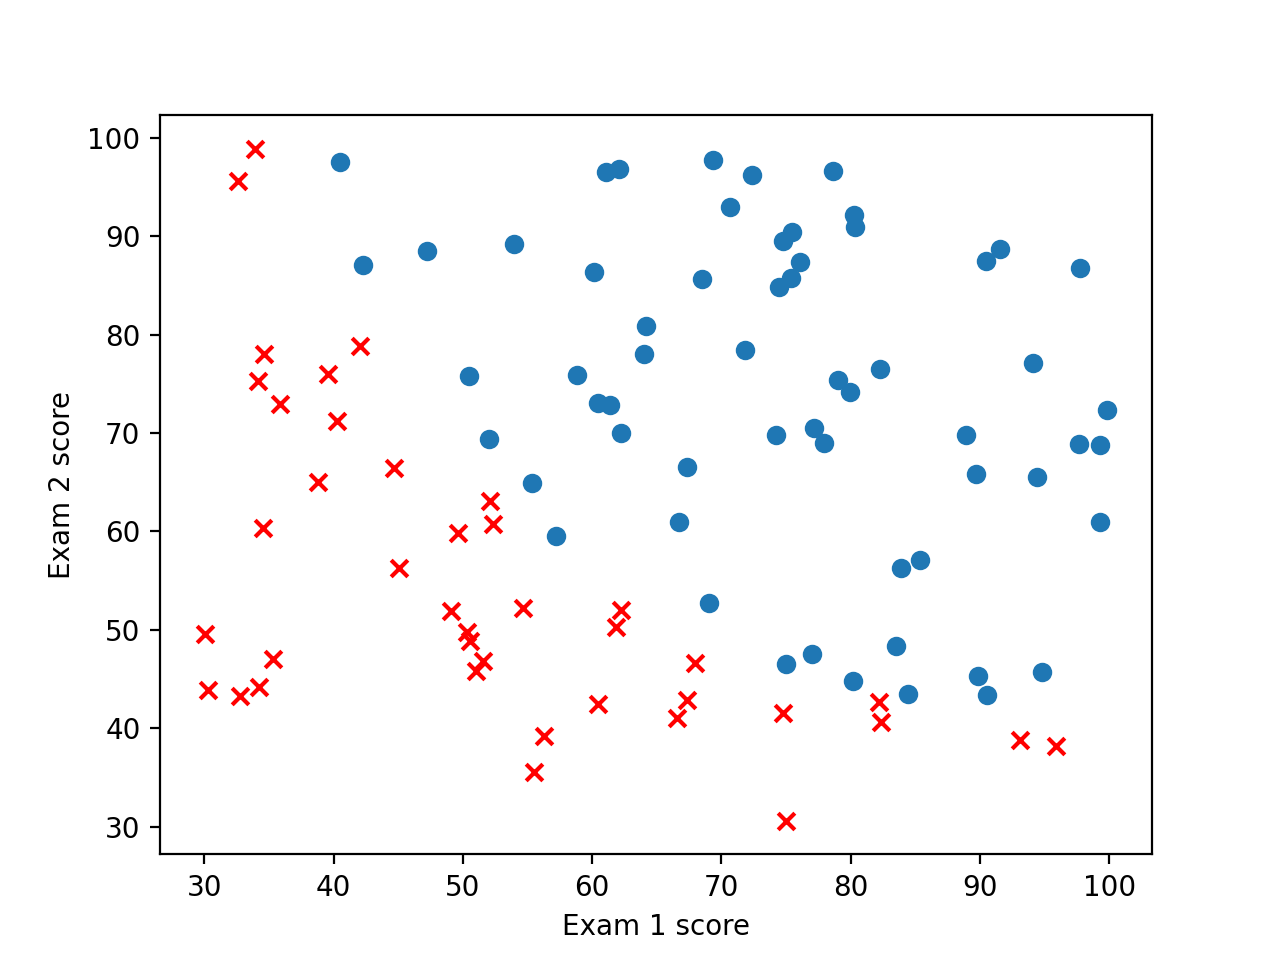
\includegraphics[width=0.5\linewidth]{figs/Chap_4_Figure_1.png}
\end{figure}

python 实现逻辑回归如下：

\begin{lstlisting}[language=Python]
import numpy as np
import matplotlib.pyplot as plt
import math

alpha = 0.01
iteration = 10000
Z = []

def Normalization(data):
	return (data - data.mean(axis = 0)) / data.std(axis = 0, ddof = 1)

def h(T, x):
	return 1 / (1 + np.e ** (-np.matmul(T.T, x)[0][0]))

def J(T, X, Y):
	res = 0
	for i in range(m):
		res -= Y[i] * math.log(h(T, X[i:i+1, :].T)) + \
		(1 - Y[i]) * math.log(1 - h(T, X[i:i+1, :].T))
	res /= m
	return res

def partJ(T, X, Y):
	res = np.zeros((n, 1))
	for i in range(m):
		res += (h(T, X[i:i+1, :].T) - Y[i]) * X[i:i+1, :].T
	res /= m
	return res

def GradientDescent(X, Y):
	T = np.zeros((n, 1))
	for t in range(iteration):
		T = T - alpha * partJ(T, X, Y)
		Z.append(J(T, X, Y))
	return T

data = np.genfromtxt("ex2data1.txt", delimiter = ',')
(m, n) = data.shape
data[:, :-1] = Normalization(data[:, :-1])
X = np.column_stack((np.ones((m, 1)), data[:, :-1]))
Y = data[:, -1]
T = GradientDescent(X, Y)
print(T)
print(J(T, X, Y))

p1 = plt.subplot(111)
p1.plot(range(1, iteration+1), Z)
p1.set_xlabel("Iteration")
p1.set_ylabel("Cost")
plt.show()
\end{lstlisting}

在学习率为 $0.01$ 下迭代了 $10000$ 次，结果为：$\theta=(1.2677702,\,3.05550587,\,2.81891901)^T$，此时 $J(\theta)=0.21065763610049573$. 决策边界的图像为：

\begin{figure}[H]
    \centering
    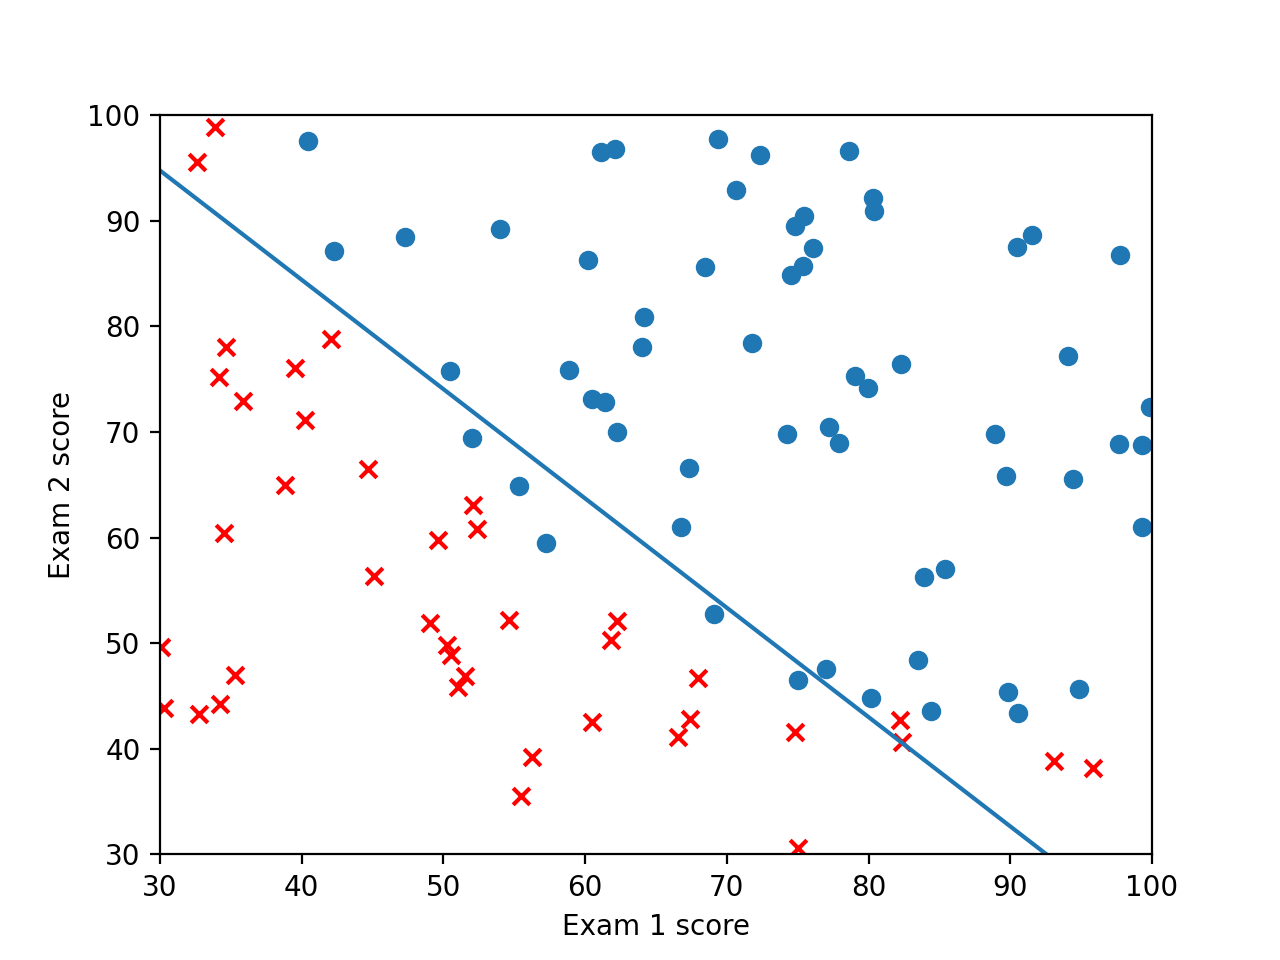
\includegraphics[width=0.5\linewidth]{figs/Chap_4_Figure_3.png}
\end{figure}

$J(\theta)$ 随迭代次数收敛情况如下：

\begin{figure}[H]
    \centering
    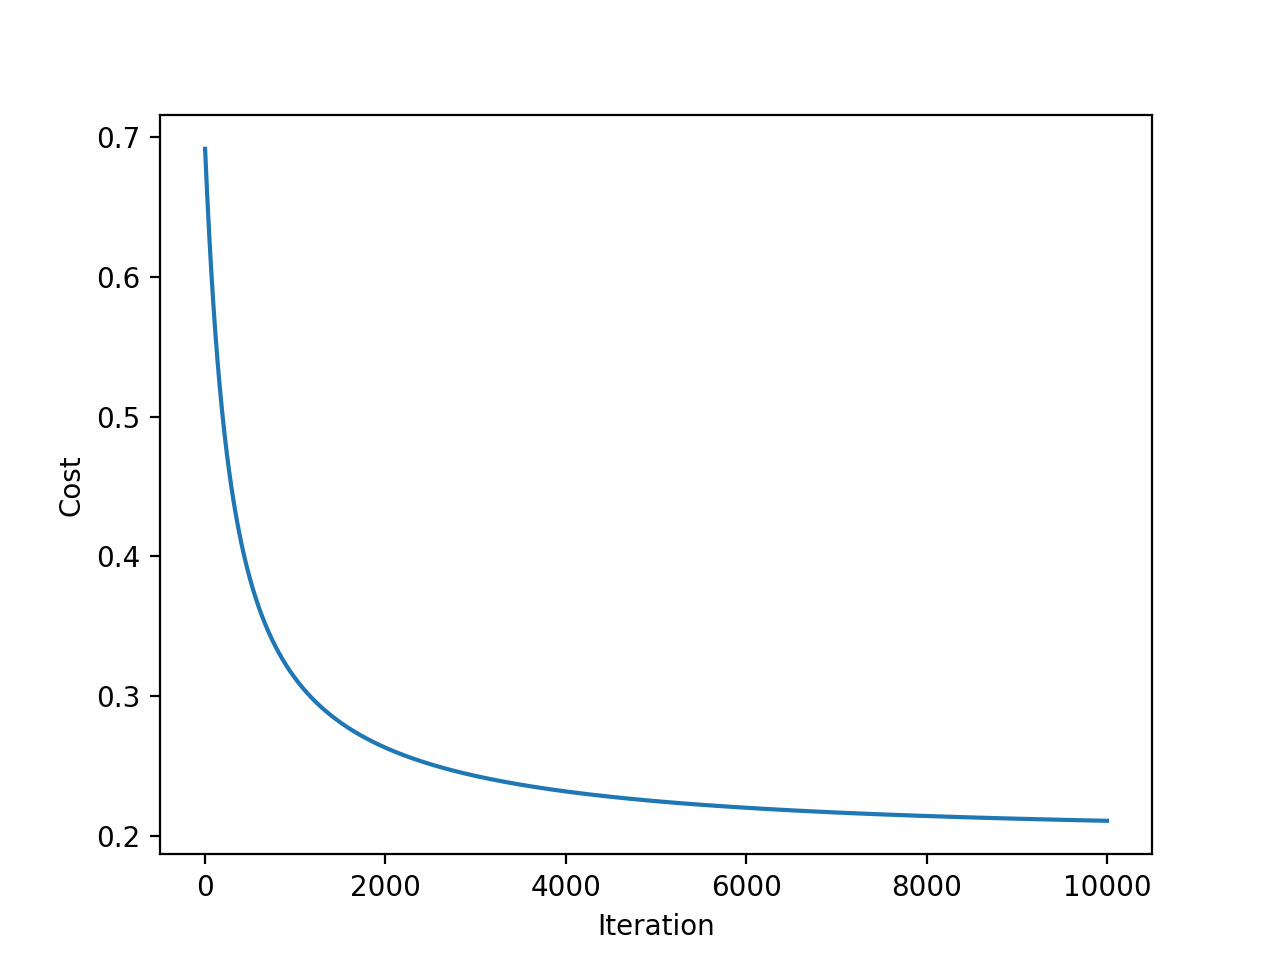
\includegraphics[width=0.5\linewidth]{figs/Chap_4_Figure_2.png}
\end{figure}
